% !TeX root = main.tex
\section{System Model}

This section describes the system model of the UAV. Some parts of this are inspired by \cite{mahony2012multirotor}. The final results (through this model) is presented in section \ref{sec:results}.

The basic system overview used is shown in figure \ref{fig:sys-overview}.

\begin{figure}[h]
    \centering
    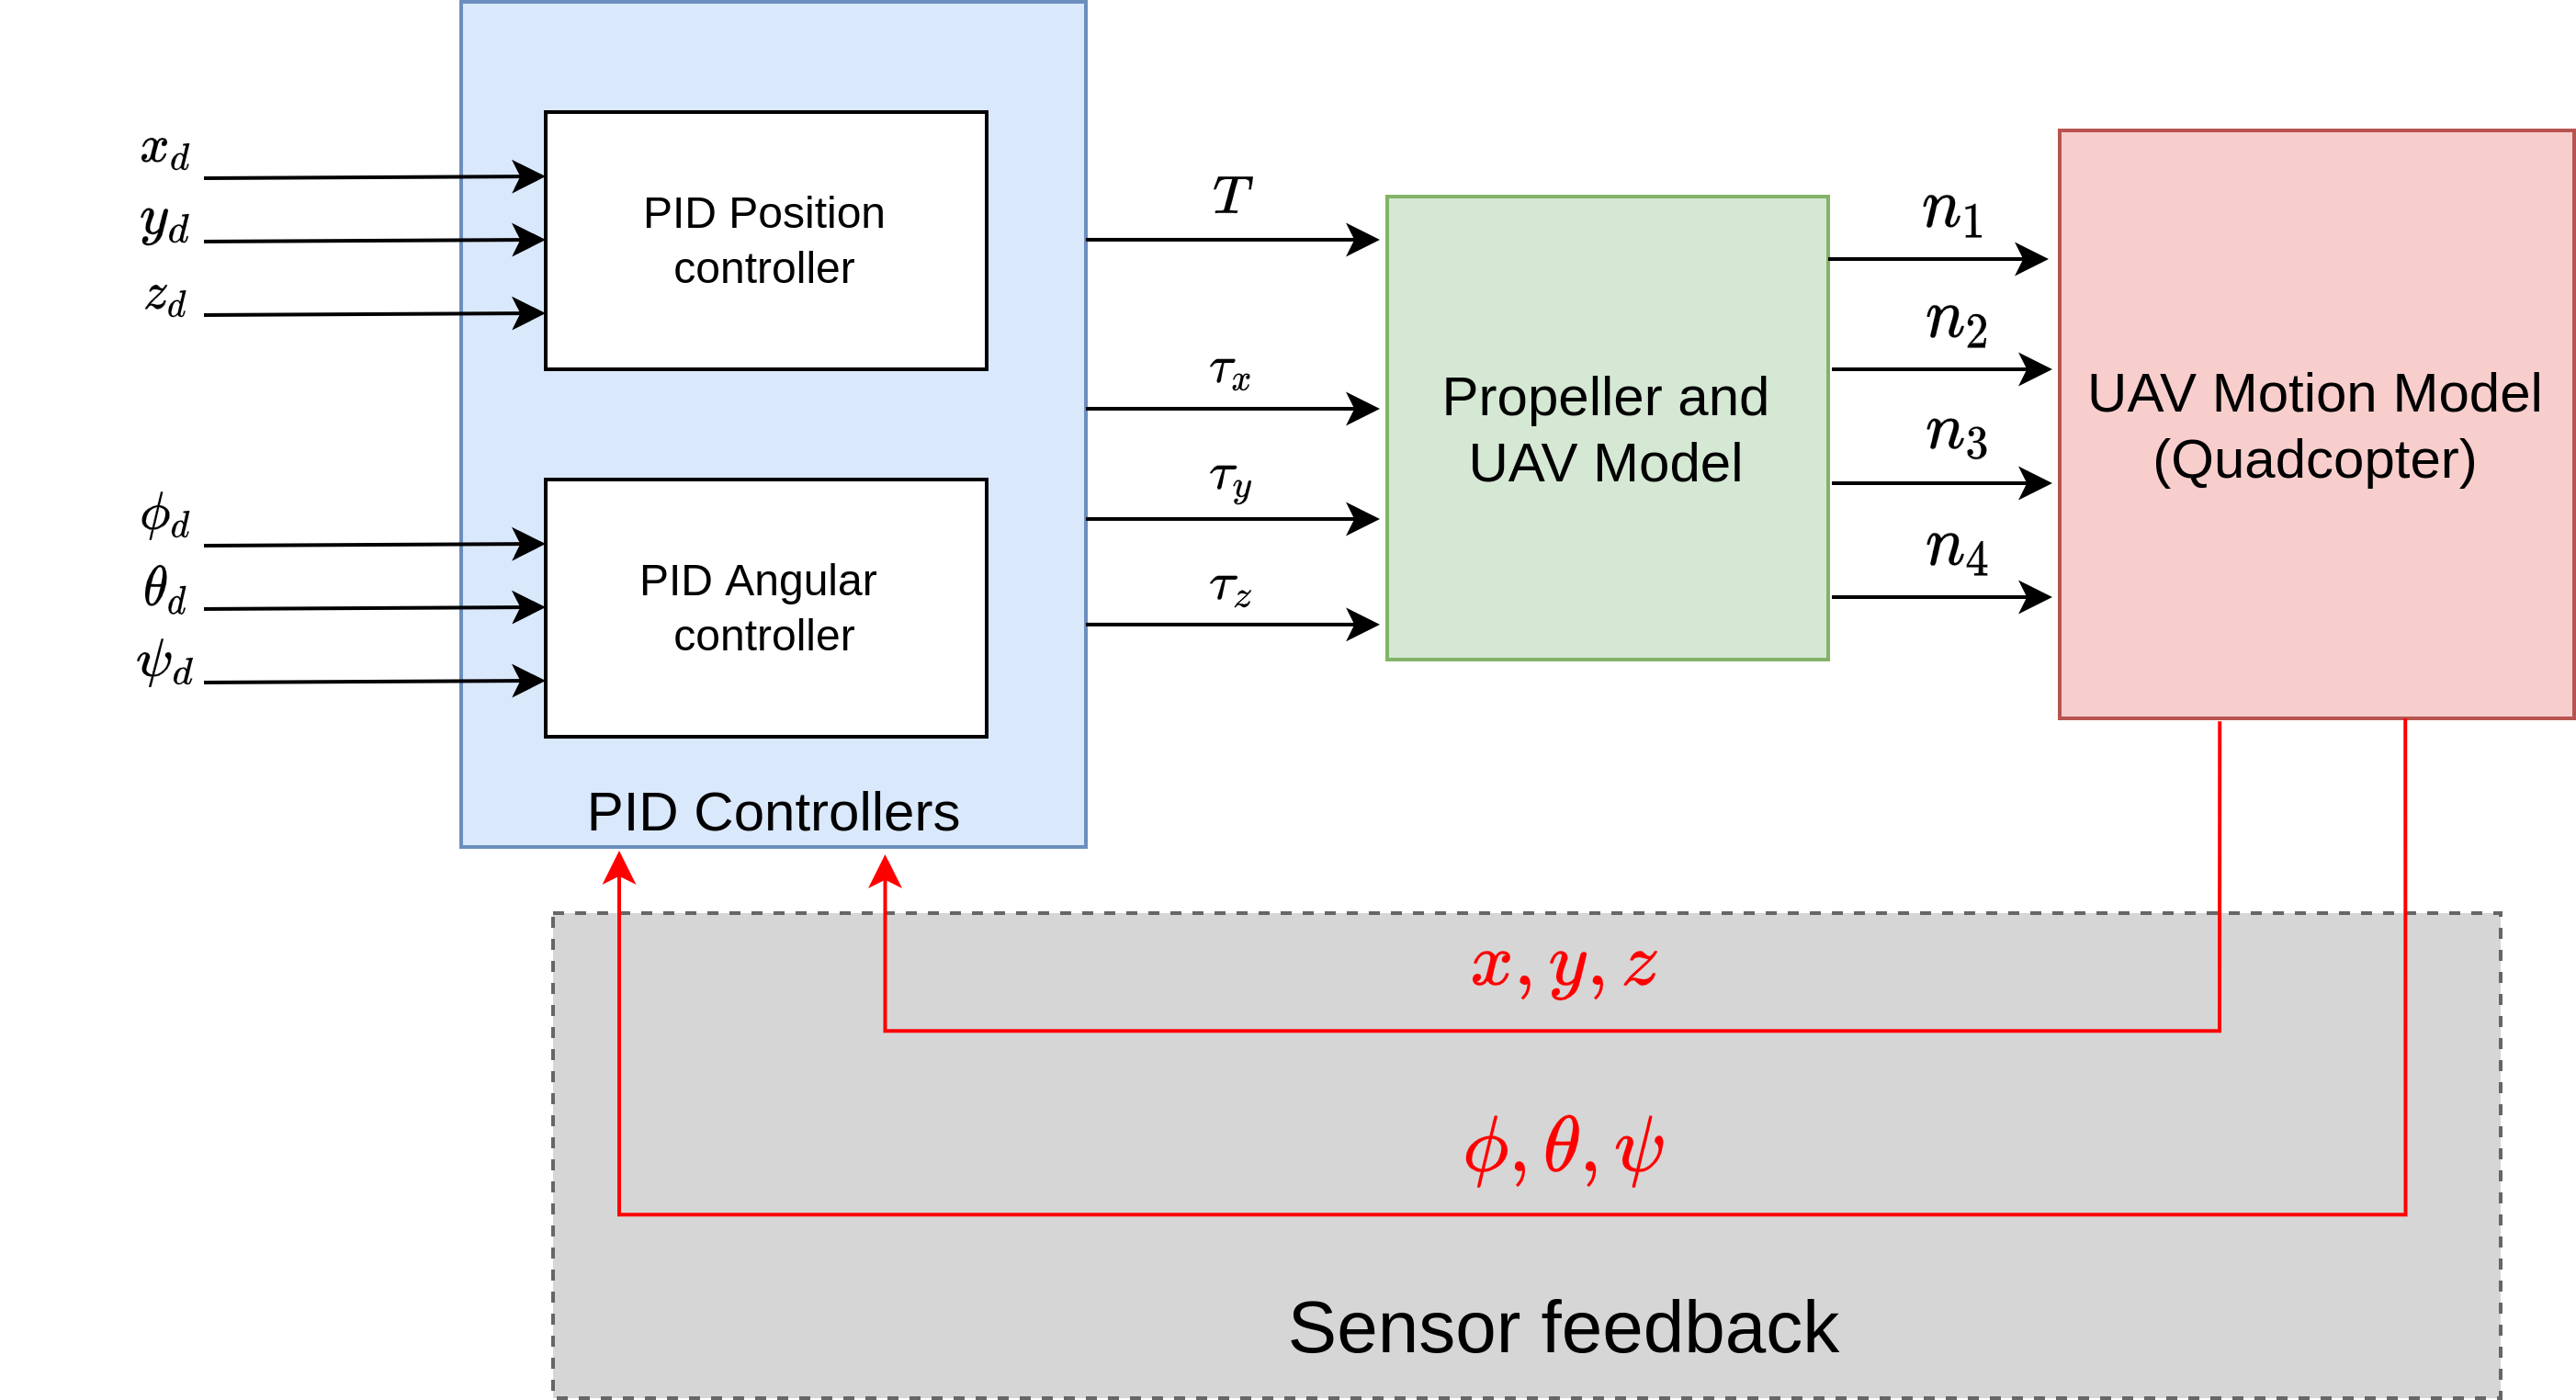
\includegraphics[width=0.9\textwidth]{uav_control_sys.png}
    \caption{UAV System overview}
    \label{fig:sys-overview}
    \small
        The PID controllers take the desired position and angles, and the current position and angles (taken through sensor data); and yield the thrust and torque action required (through predicting acceleration and using inertial model).

        The Propeller and UAV Model takes these (desired) thrust and torque actions, and converts them into (desired) propeller speed commands.

        These are given to the UAV (quadcopter). Here, we'll simulate one. Through physics (motion modeling), the new state is obtained.
\end{figure}

\subsection{PID Controllers}

There are two PID controllers. They predict the desired accelerations (control action) using PID equations. The PD controller model is described below

\begin{align}
    \mathbf{\ddot{x}} = \mathbf{k_p} (\mathbf{x_d - x}) + \mathbf{k_d} (\mathbf{\dot{x}_d - \dot{x}})
    &&
    \ddot{\alpha} = \mathbf{k_{\alpha_p}} (\alpha_d - \alpha) + \mathbf{k_{\alpha_d}} (\dot{\alpha}_d - \dot{\alpha})
\end{align}

Where $\mathbf{x} = [ x, y, z ]$ is the position and $\alpha = [ \phi, \theta, \psi ]$ is the orientation in world frame (inertial, not body).

First, we get the desired linear acceleration (and compensate for gravity). This is converted to desired thrust by multiplying with mass.

The thrust vector is converted to desired angles using knowledge of spherical angles. Basically, the thrust vector has to be aligned with the -Z axis of the UAV (that's where the propulsion is). 

The desired angles have to be \emph{clipped} (we cannot expect the UAV to fly at $90^\circ$ roll or pitch, we clip all angles received to a small angle like $20^\circ$).

The angular acceleration is calculated through the $\ddot{\alpha}$ equation above.

Angular acceleration is converted to body torques using the inertia tensor $\mathbf{J}$, that is $\tau = \mathbf{J} \ddot{\alpha} = [\tau_x, \tau_y, \tau_z]$. The thrust is already derived from $\ddot{\mathbf{x}}$ (as described above).

\subsection{Propeller equations}

Refer to the image below for getting the directional sense of propeller rotations.

\begin{figure}[ht]
    \centering
    \begin{subfigure}[b]{0.3\textwidth}
        \centering
        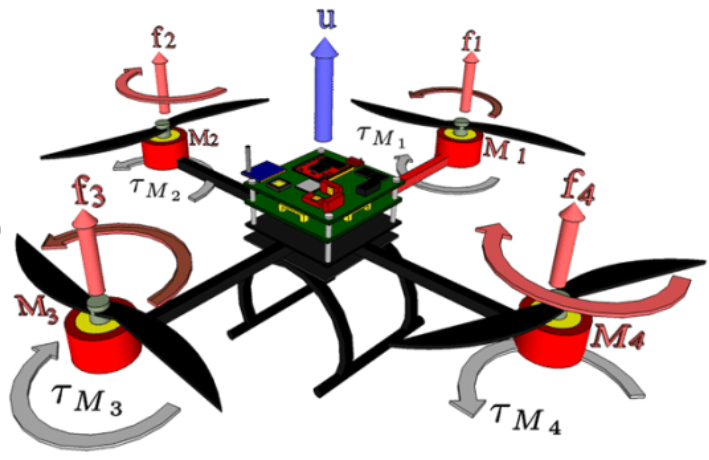
\includegraphics[width=\textwidth]{uav_prop_thrust.png}
        \caption{Thrust}
    \end{subfigure}
    \begin{subfigure}[b]{0.6\textwidth}
        \centering
        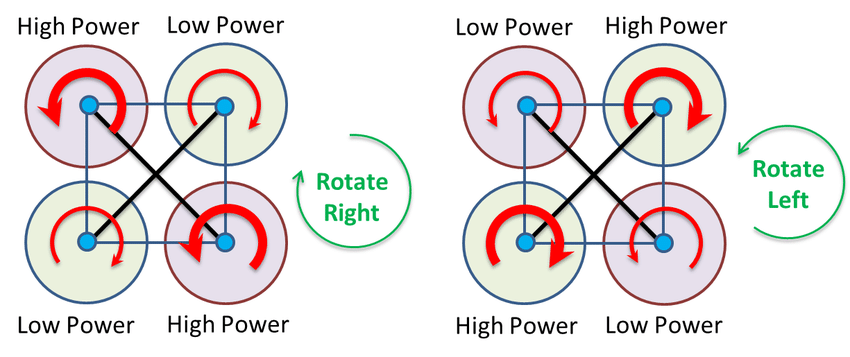
\includegraphics[width=\textwidth]{uav_yaw_ctrl.png}
        \caption{Yaw control}
    \end{subfigure}
    \caption{UAV Propeller Thrust}
    \label{fig:uav-prop-thrust}
\end{figure}

From figure \ref{fig:uav-prop-thrust}, the following system of equations are clear

\begin{equation}
    \begin{bmatrix}
    -T \\ \tau_{x_b} \\ \tau_{y_b} \\ \tau_{z_b}
    \end{bmatrix} = \underset{\mathbf{M}}{\underbrace{\begin{bmatrix}
    k_t & k_t & k_t & k_t \\
    0.5 L k_{\tau} & -0.5 L k_{\tau} & -0.5 L k_{\tau} & 0.5 L k_{\tau} \\
    0.5 L k_{\tau} & 0.5 L k_{\tau} & -0.5 L k_{\tau} & -0.5 L k_{\tau} \\
    k_{\tau} & -k_{\tau} & k_{\tau} & -k_{\tau}
    \end{bmatrix}}}
    \begin{bmatrix}
    n_1^2 \\ n_2^2 \\ n_3^2 \\ n_4^2
    \end{bmatrix}
    \label{eq:prop-thrust-fm-sp}
\end{equation}

Using equation \ref{eq:prop-thrust-fm-sp}, we can find the motor speeds $n$ (by inverting $\mathbf{M}$).

Note that we used $-T$ here because thrust, which is to counter weight, is in the -Z direction (it'll finally be positive).

A clipping for propeller speeds is also applied, the motors can only give a particular maximum rotation speed.

\subsection{UAV Motion Model}

Using the (clipped) propeller speeds $n_i$, we first get the thrust $T$ (should be -ve because it is along -Z). We represent this $T$ in the inertial frame using the relation below

\begin{equation}
    \mathbf{T}_\textup{inertial} = \underset{^i_b\mathbf{R} = \textup{R}(\textup{Z},\psi) \textup{R}(\textup{Y},\theta) \textup{R}(\textup{X},\phi)}{\underbrace{
        \begin{bmatrix}
        c_\theta c_\psi & s_\phi s_\theta c_\psi - c_\phi s_\psi & s_\phi s_\psi + c_\phi s_\theta c_\psi \\
        c_\theta s_\psi & s_\phi s_\theta s_\psi + c_\phi c_\psi & -s_\phi c_\psi + c_\phi s_\theta s_\psi \\
        -s_\theta & s_\phi c_\theta & c_\phi c_\theta
        \end{bmatrix}}
    } \; \mathbf{T}_{\textup{body}}
    \label{eq:forces-body-to-inertial}
\end{equation}

In equation \ref{eq:forces-body-to-inertial}, $\mathbf{T}_{\textup{body}} = [0\;\;0\;\;-T]^\top$ where $T$ is the (positive) thrust from propellers.

We add $[0\;\;0\;\;mg]^\top$ (weight) to $\mathbf{T}_\textup{inertial}$ and divide by $m$ to get the \emph{linear acceleration} (in world fixed/inertial frame).

We use equation \ref{eq:prop-thrust-fm-sp} to get the body torque vector $\tau = [\tau_x \;\; \tau_y \;\; \tau_z]^\top$. We use the coriolis equation below to get the angular accelerations in the body frame

\begin{equation}
    \mathbf{J} \left ( \frac{d \mathbf{\Omega}}{dt} \right )_{\textup{B}} + \mathbf{\Omega} \times (\mathbf{J \Omega}) = \tau
    \label{eq:coriolis-angacc-body}
\end{equation}

Where $\Omega$ is the angular velocity in the (get it from equation \ref{eq:angvel-body-inertial}). Using equation \ref{eq:coriolis-angacc-body}, we get the angular acceleration $\left ( \sfrac{d \mathbf{\Omega}}{dt} \right )_{\textup{B}}$.

The relation between the angular velocity in the inertial frame and the angular velocity in the body frame is given below

\begin{align}
    \mathbf{\Omega} = \begin{bmatrix}
        p \\ q \\ r
    \end{bmatrix} &= \begin{bmatrix}
        \dot{\phi} \\ 0 \\ 0
        \end{bmatrix} + \textup{Rot}(X, -\phi) \begin{bmatrix}
        0 \\ \dot{\theta} \\ 0
        \end{bmatrix} + \textup{Rot}(X, -\phi) \textup{Rot}(Y, -\theta) \begin{bmatrix}
        0 \\ 0 \\ \dot{\psi}
        \end{bmatrix}
        \nonumber \\
    &= \underset{\mathbf{M}_\Omega}{\underbrace{\begin{bmatrix}
        1 & 0 & -s_\theta \\
        0 & c_\phi & s_\phi c_\theta \\
        0 & -s_\phi & c_\phi c_\theta
        \end{bmatrix}}} \begin{bmatrix}
            \dot{\phi} \\ \dot{\theta} \\ \dot{\psi}
        \end{bmatrix}
    \label{eq:angvel-body-inertial}
\end{align}

We apply \ref{eq:angvel-body-inertial} to get $\Omega$, and then apply \ref{eq:coriolis-angacc-body} to get $\dot{\Omega}$. Angular acceleration of body frame is derived by inverting $\mathbf{M}_\Omega$ in equation \ref{eq:angvel-body-inertial}. We now have \emph{body's angular accelerations} in the inertial frame.

We use the obtained angular acceleration to update angular velocity, and subsequently the angles $[\phi\;\;\theta\;\;\psi]^\top$. We also use the obtained linear accelerations to update the body velocity and acceleration.

\subsection{Conclusion}

The above three sections are applied iteratively in a loop till the final time. Maybe drag can be added in the force calculations (for drag force of body frame in inertial frame). This submission doesn't include that.
